\documentclass{article}
\usepackage[utf8]{inputenc}
\usepackage{graphicx,amsmath,amsfonts,amssymb,caption,subcaption, subfigure}
\usepackage[font={scriptsize}]{caption}

\begin{document}
\title{SVVR Assignment 3}
\author{Sander Nugteren (6042023) \and Merel de Groot (6103677)}
\renewcommand{\today}{November 24, 2014}
\maketitle

\section*{Visualization of a Static Mixing Reactor}
The goal of the assignment is to use VTK to render a visualization of a static mixing reactor. The source of the visualization pipeline is a dataset containing scalars that represent the mixer and vectors that represent the fluid. 

Three filters are applied to the data, one to model the isosurface of the mixer and two line tracers to model each fluid. Each line tracer has their own center from which the lines originate to show how two colours get mixed through the mixer. Then tubes are assigned to these lines to add thickness to make them visible.  

Next, all filters are assigned to their own mapper to set the graphical primitives and then passed on to an actor. For colouring the mapper stage is set to ignore scalar values, giving the color as a argument of the actor. Finally these actors are combined in one renderer. 

\section*{Results}
\subsection*{The morphology of the reactor}
For the morphology of the reactor, only the isosurface is depictured, on a lighter background. The images shown by \ref{mixerMorph} show the structure of the mixer. The image on the right shows that the beams of the structure have spikes to disperse the fluids more efficiently for mixing.

\begin{figure}[ht]
\centering
\subfigure[Top view]
{
\includegraphics[width=3.8cm]{SVVR_mixerTop.png}}
\subfigure[From front to side view]
{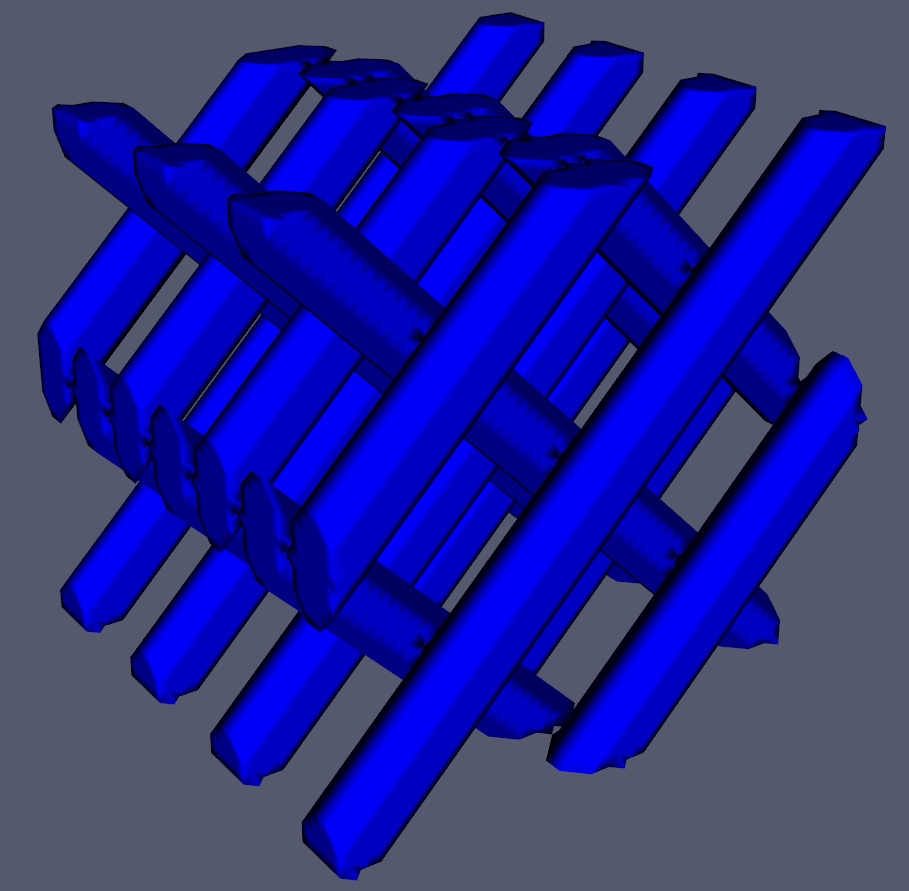
\includegraphics[width=3.8cm]{SVVR_mixerSide.png}}
\subfigure[Side view]
{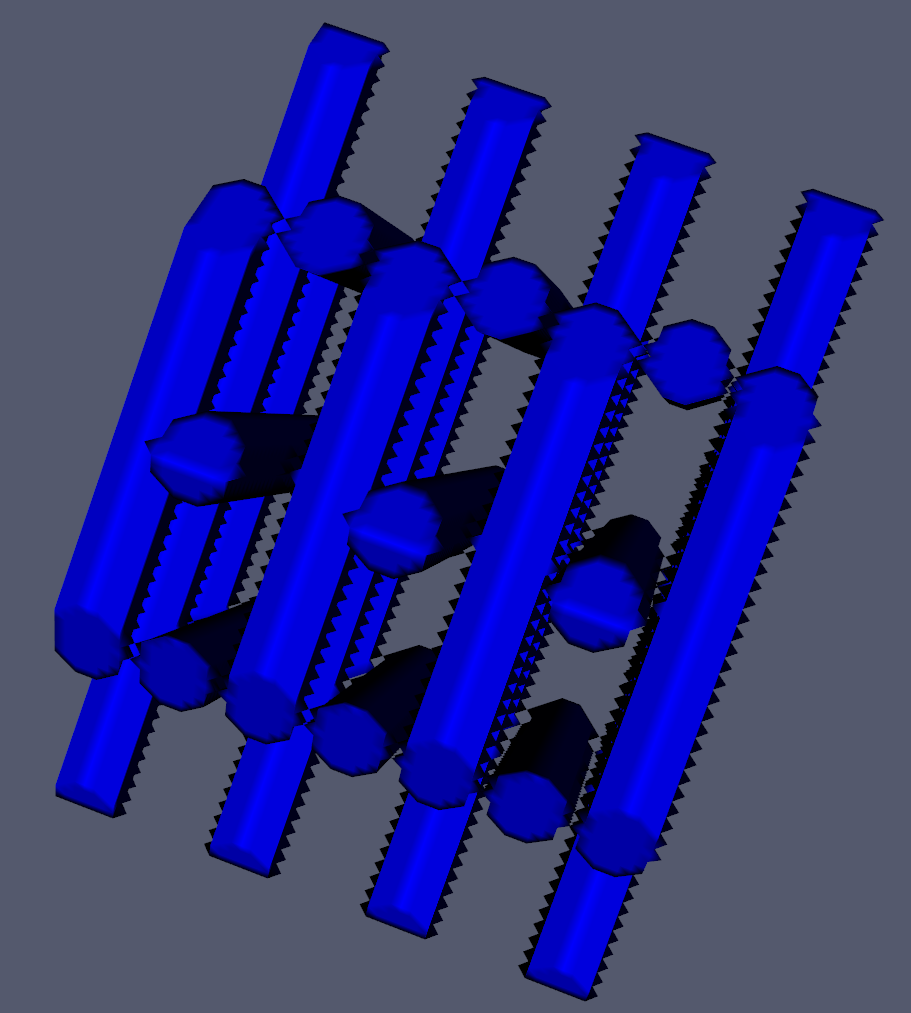
\includegraphics[width=3.8cm]{SVVR_mixerSpikes.png}}
\caption{The mixer from multiple angles to show its 3D structure.}
\label{mixerMorph}
\end{figure}  

\newpage
\subsection*{The capability of the reactor to mix two fluids}
To show whether the mixer is capable of mixing the two fluids, all three filters are depicted in the left image of figure \ref{fluids}. This top view shows that the fluids are injected seperately on the left side and are mixed on the right side, after going through the mixer. To show more accurately what happens within the mixer, the right image shows the same view, but without the mixer. This image shows that the mixer is capable of mixing the two fluids.

\begin{figure}[ht]
\centering
\subfigure[The mixer with the two fluids]
{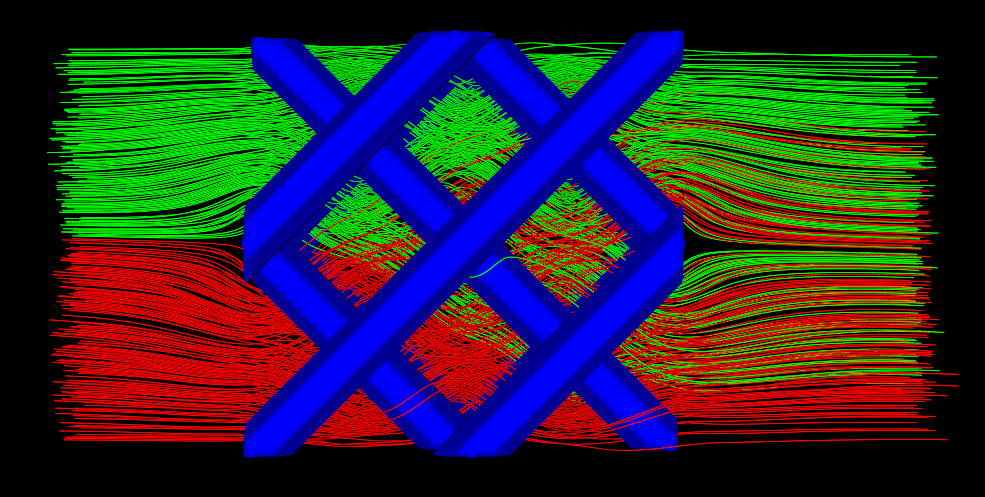
\includegraphics[width=6cm]{SVVR_mixer.png}}
\subfigure[The fluids]
{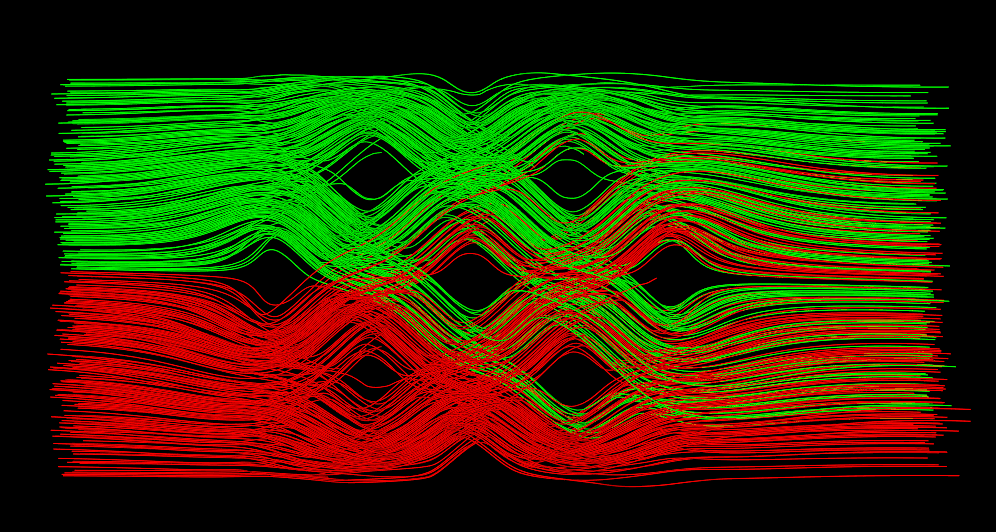
\includegraphics[width=6cm]{SVVR_fluids.png}}
\caption{The mixing of the fluids, shown with and without the mixer.}
\label{fluids}
\end{figure}  

\subsection*{The flow velocity around the reactor}



\end{document}


